%%================================================
%% File: main.tex
%% Encoding: UTF-8
%% Author: Yuan Xiaoshuai - yxshuai@gmail.com
%% Created: 2017-05-25 10:18
%% Last modified: 2019-11-14 22:10
%%================================================
\documentclass[degree=doctor]{ucasthesis}
% \documentclass[degree=doctor]{ucasthesis}
% 选项:
%   degree=[master|doctor],                   % 必选
%   secret,                                   % 可选
%   mkshuji,                                  % 可选
% 注意:mkshuji 选项需要系统中安装 Noto Sans CJK SC 字体

% 所有其它可能用到的包都统一放到这里了,可以根据自己的实际添加或者删除。
\usepackage{ucasthesis}

% 定义所有的图片文件在 figures 子目录下
\graphicspath{{figures/}}

% 可以在这里修改配置文件中的定义。导言区可以使用中文。
% \def\myname{赵钱孙}

\begin{document}

%%% 封面部分
\frontmatter
%%================================================
%% File: cover.tex
%% Encoding: UTF-8
%% Author: Yuan Xiaoshuai - yxshuai@gmail.com
%% Created: 2017-05-25 10:18
%% Last modified: 2019-11-14 16:05
%%================================================
\ucassetup{
  %******************************
  % 注意:
  %   1. 配置里面不要出现空行
  %   2. 不需要的配置信息可以删除
  %******************************
  %
  %=========
  % 中文信息
  %=========
  ctitle={中国科学院大学学位论文 \LaTeX\ 模板\\使用示例文档 v\version},
  ctitlemark={中国科学院大学学位论文 LaTeX 模板使用示例文档 v\version},
  cdegree={工学博士},
  cdepartment={中国科学院大连化学物理研究所},
  cmajor={化学工程},
  cauthor={赵钱孙},
  csupervisor={吴郑王\hspace{2\ccwd}教\hspace{\ccwd}授},
  csupervisorplace={中国科学院大连化学物理研究所},
  ccosupervisor={李\hspace{\ccwd}周\hspace{2\ccwd}研究员}, % 辅助老师
  % 日期自动使用当前时间,若需指定按如下方式修改:(夏季毕业填写6月,冬季填写12月)
  cdate={2018 年 6 月},
  % 致谢日期
  ackdate={2018 年 6 月于某地}, 
  %
  %=========
  % 英文信息
  %=========
  etitle={An Introduction to \LaTeX{} Thesis\\ Template of University of Chinese Academy of Sciences\\ v\version},
  etitlemark={An Introduction to LaTeX Thesis Template of University of Chinese Academy of Sciences v\version},
  edegree={Doctor of Engineering},
  emajor={Chemical Engineering},
  eauthor={Qiansun Zhao},
  esupervisor={Professor Zhengwang Wu},
  ecosupervisor={Professor Zhou Li},
  edepartment={Dalian Institute of Chemical Physics, Chinese Academy of Sciences},
  % 日期自动生成,若需指定按如下方式修改:
  edate={June, 2018}
}
% %%================================================
%% Filename: ack.tex
%% Encoding: UTF-8
%% Author: Yuan Xiaoshuai - yxshuai@gmail.com
%% Created: 2012-01-12 18:09
%% Last modified: 2016-08-28 21:05
%%================================================
\begin{ack}

韶华易逝,光阴荏苒,余自入渝倏忽而又三年矣。曩者,离鲁地,弃吴越奔巴蜀,恢恢乎
若漏网之鲫,惶惶乎似惊弓之鸟,几无容身之地。幸遇刘徐二相荐,得拜于恩师魏公门下
,而今已历六秋。先生治学严谨,博通中外,蔚为家,研习学术,废寝忘食,已臻忘我之
境界。犹忆当年,乍入门墙,耻无寸功先生不以余愚钝,委以重托,是以矢勤矢勇,思惟
速战,毋负所托。然欲速不心忧如焚。全赖先生数次点拨,每自躬亲,甚于子夜,共为进
退,方有所成。于缀词成文,苦心孤诣,字斟句酌,独具匠心,深为叹服,并于耳提面命
之际益良多。先生之德才,若高山仰止,亦非庸庸如吾辈者所能望其项背。每至周常言:
“修身者智之府也,爱施者仁之端也,取予者义之符也,耻辱者勇之决也立名者行之极也
。凡此五者,皆安身立命之本,不可偏废。”言之谆谆,听之诚若醍醐灌顶。退而思之,
果斯然也,大为拜服。兼之师母,待余恩厚,视若螟多得给养,感激涕零。余素朴陋,尚
无剖符丹书之功,反受此殊遇,非结草衔不可报也!今虽即辞师门,必常怀乌鸟之情,反
哺之心,诚不失其望也!

师门同侪,学强张骞,皆忠义之士,情同手足;乐至四国,许都耀琼,此良实,多蒙所助
;兰莉二姊,性行淑均,爱如姐弟。其他诸君,皆为志虑忠纯士,多有广益。区区不才,
有何德能,安得广助若此?感荷之心,亦自拳拳。实验中曾多次求教于杨(明莉)、杜(
军)二老师,受益匪浅;中心实验室(光辉)、鲜(晓红)二位老师及刘姊渝萍为实验工
作大开方便之门,谨表谢忱家中上至期颐之祖母,中至慈爱之父母、姊姊,下至始龀之甥
男,均不遗力以支持,融融亲情,曷其幸甚!谨撰此文,鱼传尺素,答报椿萱!

嗟乎!聚散无常,盛况难再;书不尽意,略陈固陋。临别赠言,幸承恩于公;登高作赋,
是所望于群贤。斗胆献拙,情之不已;一言均赋,四韵俱成。洒陵江,以酹逝去之岁月。

\begin{center}
西入渝州已六霜,貔貅帐里铸鱼肠。\\
书山文海研学术,翠袖红巾戏皮黄。\\
莫叹时舛惟虎踞,且图运转季鹰扬。\\
今朝叩别师尊去,一片丹心化碧江。
\footnote{重庆大学化工博士季孟波学位论文《抗溺水性气体多孔电极的研究》致谢词}
\end{center}

\end{ack}

%%================================================
%% Filename: abstract.tex
%% Encoding: UTF-8
%% Author: Yuan Xiaoshuai - yxshuai@gmail.com
%% Created: 2012-04-24 00:21
%% Last modified: 2019-11-10 10:26
%%================================================
\begin{cabstract}

% 作者所在研究所要求中文摘要内容不能超过一页,稍微多于一页时可以调整行距实现
% \xiaosi[1.72] % fit the abstract in one page

\ucasthesis{}(中国科学院大学学位论文模板)提供中国科学院大学研究生学位论文的模板,代码来源于清华大学学位论文模板(\textsc{ThuThesis}),并根据中国科学院大学学位论文写作规范格式的要求进行了修改。该模板为作者撰写博士论文所用,且通过了格式审查,但由于国科大各研究院所对格式的要求可能存在差异,可能需要根据具体研究院所的格式要求进行一定的调整。

本文的创新点主要有:

  \begin{itemize}
    \item 用例子来解释模板的使用方法;
    \item 用废话来填充无关紧要的部分;
    \item 一边学习摸索一边编写新代码。
  \end{itemize}

\textsf{模板作者注}:关键词分隔符用半角逗号,模板会自动处理替换为《规范》中
规定的分隔符,英文关键词同理。

\end{cabstract}

\ckeywords{TeX/LaTeX, XeLaTeX与中文处理, 科技排版, 国科大, 学位论文
模板, 关于摘要}

\begin{eabstract} 

An abstract of a dissertation is a summary and extraction of research work and
contributions. Included in an abstract should be description of research topic
and research objective, brief introduction to methodology and research
process, and summarization of conclusion and contributions of the research. An
abstract should be characterized by independence and clarity and carry
identical information with the dissertation. It should be such that the
general idea and major contributions of the dissertation are conveyed without
reading the dissertation. 

\end{eabstract}

\ekeywords{TeX/LaTeX, XeLaTeX Chinese, Scientific typesetting system,
Academic thesis template, UCAS, About keywords}



\makecover

%% 目录
\tableofcontents
\listoffigures* % 星号表示不在目录中显示图表目录
\listoftables*

%% 符号对照表
% 规范未限定放置顺序,但研究生部要求放文后
% 鉴于各研究院所要求不同,可以试着放前面,页眉页脚会自动调整
% %%================================================
%% Filename: denotation.tex
%% Encoding: UTF-8
%% Author: Yuan Xiaoshuai - yxshuai@gmail.com
%% Created: 2012-01-14 13:44
%% Last modified: 2019-11-05 15:46
%%================================================
\begin{denotation}

\item[HPC] 高性能计算 (High Performance Computing)
\item[cluster] 集群
\item[Itanium] 安腾
\item[SMP] 对称多处理
\item[API] 应用程序编程接口
\item[PI]	聚酰亚胺
\item[MPI]	聚酰亚胺模型化合物,N-苯基邻苯酰亚胺
\item[PBI]	聚苯并咪唑
\item[MPBI]	聚苯并咪唑模型化合物,N-苯基苯并咪唑
\item[PY]	聚吡咙
\item[PMDA-BDA]	均苯四酸二酐与联苯四胺合成的聚吡咙薄膜
\item[$\Delta G$]  	活化自由能~(Activation Free Energy)
\item [$\chi$] 传输系数~(Transmission Coefficient)
\item[$E$] 能量
\item[$m$] 质量
\item[$c$] 光速
\item[$P$] 概率
\item[$T$] 时间
\item[$v$] 速度
\item[劝学] 君子曰:学不可以已。青,取之于蓝,而青于蓝;冰,水为之,而寒于水。
木直中绳。(车柔)以为轮,其曲中规。虽有槁暴,不复挺者,(车柔)使之然也。故木
受绳则直, 金就砺则利,君子博学而日参省乎己,则知明而行无过矣。吾尝终日而思矣
,  不如须臾之所学也;吾尝(足齐)而望矣,不如登高之博见也。登高而招,臂非加长
也,  而见者远;  顺风而呼,  声非加疾也,而闻者彰。假舆马者,非利足也,而致千
里;假舟楫者,非能水也,而绝江河,  君子生非异也,善假于物也。积土成山,风雨兴
焉;积水成渊,蛟龙生焉;积善成德,而神明自得,圣心备焉。故不积跬步,无以至千里
;不积小流,无以成江海。骐骥一跃,不能十步;驽马十驾,功在不舍。锲而舍之,朽木
不折;  锲而不舍,金石可镂。蚓无爪牙之利,筋骨之强,上食埃土,下饮黄泉,用心一
也。蟹六跪而二螯,非蛇鳝之穴无可寄托者,用心躁也。——荀况
\end{denotation}


%%% 正文部分
\mainmatter
%%================================================
%% Filename: chap01.tex
%% Encoding: UTF-8
%% Author: Yuan Xiaoshuai - yxshuai@gmail.com
%% Created: 2019-11-10 10:30
%% Last modified: 2020-11-26 01:28
%%================================================
\chapter{模板简介及使用说明 Introduction}
\label{cha:introduction}

\ucasthesis{}(\textbf{U}niversity of the \textbf{C}hinese \textbf{A}cademy of \textbf{S}ciences \LaTeX{} \textbf{Thesis} Template) 是中国科学院大学研究生学位 \LaTeX{} 论文模板,根据清华大学学位论文模板(\textbf{thuthesis})修改而来。

本文档将尽量完整的介绍模板的使用方法,并给出示例。如有不清楚之处可以向作者提问,也非常欢迎有兴趣者共同完善此模板。

\section{模板安装及编译运行}
\label{sec:install}

该模板可以在项目 \href{https://github.com/tuxify/ucasthesis}{\emph{GitHub 主页}} 下载 \href{https://github.com/tuxify/ucasthesis/releases}{\textbf{发布版本}} 或者 \href{https://codeload.github.com/tuxify/ucasthesis/zip/master}{\textbf{开发版本}}。下载后进入模板主目录即可编译生成示例文档,模板在 \TeXLive{} 2019 下编译通过,建议采用最新版本的 \TeXLive{} 软件发行套装 \footnote{软件的安装参见:\url{http://tug.org/texlive/acquire.html}}。示例文档的生成有很多种方法,这里分别给出手动逐条运行命令和采用自动运行脚本两种编译方法的示例。

手动运行时,需要多次运行编译指令,直到不再出现警告为止。根据所采用的参考文献后端,需要执行不同的命令。采用 \texttt{bibtex} 处理参考文献时,需运行如下命令:
\begin{description}
  \item[\$] xelatex main
  \item[\$] bibtex main
  \item[\$] xelatex main
  \item[\$] xelatex main
\end{description}

采用 \texttt{biblatex} 处理参考文献时,需运行如下命令:
\begin{description}
  \item[\$] xelatex main
  \item[\$] biber main
  \item[\$] xelatex main
  \item[\$] xelatex main
\end{description}

自动运行则可以采用 latexmk 命令全自动生成文档,该命令会自动运行多次工具直到交叉引用都被解决。需运行的命令如下:
\begin{description}
  \item[\$] latexmk -xelatex main
\end{description}

模板作者使用的开发环境是 \emph{Visual Studio Code 编辑器 + LaTeX Workshop 插件} 的组合工具,可以配置使用 \texttt{latexmk} 命令一键编译,具体配置方法可以参考网上的相关教程。

\section{封面相关}
\label{sec:cover}

封面的例子请参看 \texttt{data} 目录下的 \texttt{cover.tex},直接修改相关的配置即可,不需要的命令可以删除或者注释掉,里面的命令都很直观,一看即会。其它文件也类似,摘要参见 \texttt{abstract.tex},主要符号表 \texttt{nomenclature.tex},正文章节 \texttt{chap01.tex} 和 \texttt{chap02.tex},附录 \texttt{app01.tex} 和 \texttt{app02.tex},致谢\texttt{ack.tex} 个人简历 \texttt{resume.tex}。其中正文章节和附录均可新增文件,之后添加到 \texttt{main.tex} 文件相应部分即可。

\section{字体字号}
\label{sec:font}

模板默认使用 \CTeX\ 的字体配置,字体切换及字号命令可以参考 \CTeX\ 文档。此外,模板还定义了一系列字号命令,如下表所示。

\begin{center}
  \begin{tabular}{llllll}
    \toprule
    \texttt{chuhao} & \texttt{xiaochu} & \texttt{yihao}  & \texttt{xiaoyi}    & \texttt{erhao}  & \texttt{xiaoer}\\
    \texttt{sanhao} & \texttt{xiaosan} & \texttt{sihao}  & \texttt{banxiaosi} & \texttt{xiaosi} & \texttt{dawu}\\
    \texttt{wuhao}  & \texttt{xiaowu}  & \texttt{liuhao} & \texttt{xiaoliu}   & \texttt{qihao}  & \texttt{bahao}\\
    \bottomrule
  \end{tabular}
\end{center}

使用方法为:\verb|\command[<num>]|,其中 \texttt{command} 为字号命令,\texttt{num} 为行距。比如 \verb|\xiaosi[1.5]| 表示选择小四字体,行距 1.5 倍。

\section{插图表格}
\label{sec:fig_tab}

为了满足规范对插图和表格标题采用中英文双语的要求,模板调用 \textbf{bicaption} 宏包实现,并对格式部分进行了定制,用法为:
\begin{verbatim}
  \bicaption{<中文标题>}
            {<英文标题>}
  \label{<标签>}
\end{verbatim}
具体可参见第 \ref{cha:examples} 章的示例,并可查阅该宏包文档了解更多用法。

\section{参考文献}
\label{sec:ref}

模板同时支持 \textbf{bibtex} 和 \textbf{biblatex}(\textbf{biber})生成参考文献,可以根据需要选择。其中,\textbf{bibtex} 通过 \texttt{ucasthesis-author-year.bst} 和 \texttt{ucasthesis-numeric.bst} 分别提供著者-出版年制和顺序编码制的引用风格。由于 \textbf{gbt7714} 项目提供的文献风格中,支持国科大的选项尚处于开发阶段,本模板所提供的两个文件基于现有开发版中 \texttt{gbt7714-plain.bst} 和 \texttt{gbt7714-unsrt.bst} 进行了部分修改,以期尽可能满足国科大的参考文献格式。

\textbf{biblatex} 方式则采用 \texttt{biblatex-gb7714-2015} 分别提供两种引用模式的支持,并通过 \texttt{natbib} 选项保证文献调用命令与 \textbf{bibtex} 方法兼容。当采用著者-出版年制时,建议的命令为 \verb|\citet| 和 \verb|\citep|;采用顺序编码制时,建议的命令为 \verb|\cite| 和 \verb|\inlinecite|。相关示例请参见第 \ref{cha:examples} 章。

\section{其它命令}
\label{sec:other}

\subsection{书脊}

模板定义了生成书脊的命令 \verb|\shuji[<标题>][<作者>][<学校名称>]|,默认参数为论文中文题目、作者及学校名称。在论文选项中选择 \texttt{mkshuji} 选项可以直接在封面页后根据默认参数生成书脊,有需要的可以自行定制。

\emph{注意:该选项需要系统安装 Noto Sans CJK SC 字体。}

\subsection{符号列表}

示例文件中,给出了手动输入主要符号列表的方法,另外还可以通过 \textbf{nomencl} 宏包生成,即在导言区设置:
\begin{verbatim}
  \usepackage{nomencl}
  \makenomenclature
\end{verbatim}
然后在正文中任意位置使用 \verb|\nomenclature| 声明需要添加到主要符号表的符号:
\begin{verbatim}
  \nomenclature{<符号>}{<对应解释>}
\end{verbatim}
最后使用 \verb|\printnomenclature| 命令生成符号表。更详细的使用方法参见 \textbf{nomencl} 宏包的文档。
%%================================================
%% Filename: chap02.tex
%% Encoding: UTF-8
%% Author: Yuan Xiaoshuai - yxshuai@gmail.com
%% Created: 2019-11-10 10:32
%% Last modified: 2019-11-20 10:49
%%================================================
\chapter{模板使用示例 Some Examples}
\label{cha:examples}

\section{插图示例}
\label{sec:figure}

\subsection{插入单幅图形}

插图通常需要占据大块空白,所以在文字处理软件中用户经常需要调整插图的位置。
\LaTeX~有一个 \texttt{figure} 环境可以自动完成这样的任务,这种自动调整位置的环
境称作浮动环境(float),之后还会介绍表格浮动环境。

单张图片插入形式如图~\ref{fig:golfer}~所示。
\begin{figure}[htbp]
\centering
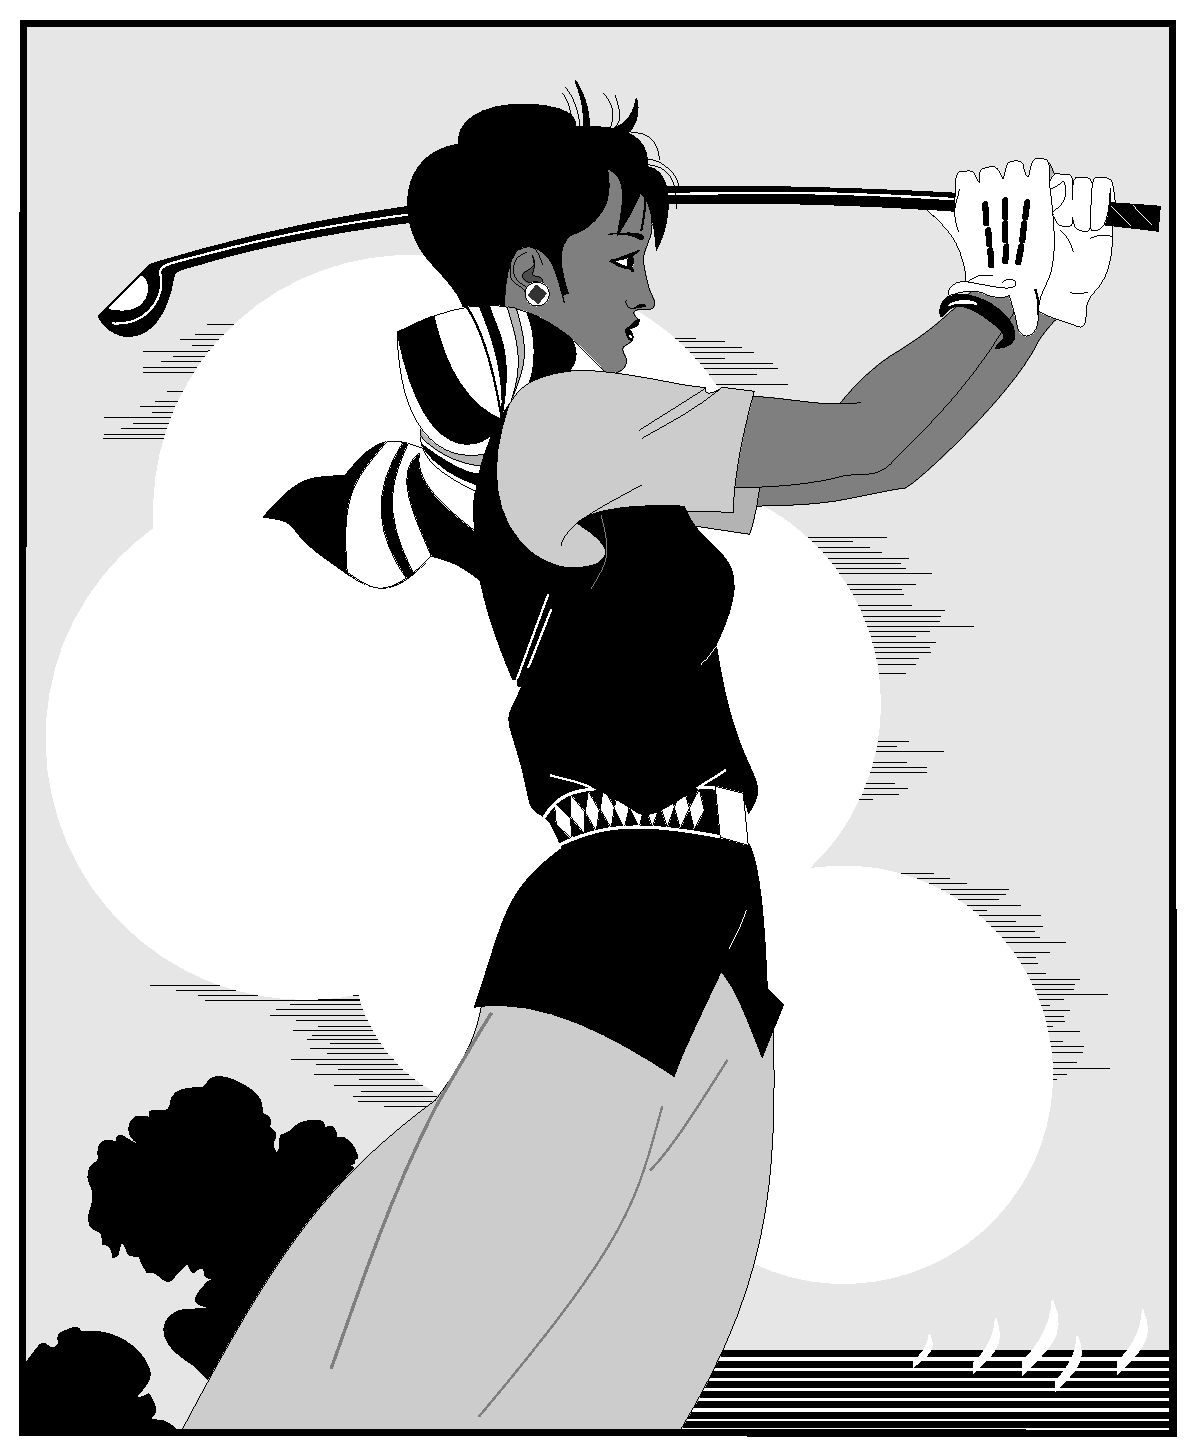
\includegraphics[width = 0.3\textwidth]{golfer}
\bicaption{打高尔夫球的人}
          {Golfer}
\label{fig:golfer}
\end{figure}

\subsection{插入多幅图形}

\subsubsection*{并排摆放,共享标题}

当我们需要两幅图片并排摆放,并共享标题时,可以在 \texttt{figure} 环境中使用两个
插图命令,如图~\ref{fig:fanqingfuming}~所示。

\begin{figure}[htbp]
\centering

\includegraphics[width=0.3\textwidth]{qingming}
\hspace{36pt}

\includegraphics[width=0.3\textwidth]{fanfu}
\bicaption{反清复明}{Fan Qing Fu Ming}
\label{fig:fanqingfuming}
\end{figure}

\subsubsection*{并排摆放,各有标题}

如果想要两幅并排的图片各有自己的标题,可以在 \texttt{figure} 环境中使用两个
 \texttt{minipage} 环境,每个环境里插入一个图,如图~\ref{fig:qingming}~和
~\ref{fig:fanfu}~所示。

\begin{figure}[htbp]
\centering
\begin{minipage}[t]{0.3\textwidth}
    \centering
    
\includegraphics[width=\textwidth]{qingming}
    \bicaption{清明}{Qing Ming}
    \label{fig:qingming}
\end{minipage}
\hspace{36pt}
\begin{minipage}[t]{0.3\textwidth}
    \centering
    
\includegraphics[width=\textwidth]{fanfu}
    \bicaption{反复}{Fan Fu}
    \label{fig:fanfu}
\end{minipage}
\end{figure}

\subsubsection*{并排摆放,共享标题,各有子标题}

如果想要两幅并排的图片共享一个标题,并各有自己的子标题,可以使用 \textbf{subcaption} 宏包提供的 \texttt{subcaptionbox} 命令,每个子图可以有各自的引用,如图~\ref{fig:subfig_a}~和~\ref{fig:subfig_b}~所示。

\begin{figure}[htbp]
\centering
\bisubcaptionbox{清明\label{fig:subfig_a}}{Qing Ming}[0.3\textwidth]{
    
\includegraphics[width=0.3\textwidth]{qingming}
}
\hspace{36pt}
\bisubcaptionbox{反复\label{fig:subfig_b}}{Fan Fu}[0.3\textwidth]{
    
\includegraphics[width=0.3\textwidth]{fanfu}
}
\bicaption{反清复明}{Fan Qing Fu Ming}
\end{figure}

\section{表格示例}
\label{sec:table}

\subsection{普通表格的绘制方法}

\texttt{table} 环境是一个将表格嵌入文本的浮动环境,其标题和交叉引用的用法类似
于上一节提到的图形浮动环境 \texttt{figure},该环境提供了最简单的表格功能。

科技文献中常使用三线表格,因此需要调用 \textbf{booktabs} 宏包,其标准格式如表~\ref{tab:booktabs}~所示。除了用该宏包所提供的命令外,模板还定义了命令 \verb|\hlinewd|,可以用于简单表格。

\begin{table}[htbp]
\bicaption{文献类型和标识代码}
          {Bibliography and Identification Code}
\label{tab:booktabs}
\centering
\begin{tabular}{cccc}
\toprule
文献类型 & 标识代码 & 文献类型 & 标识代码\\
\midrule
普通图书 & M &  会议录 & C\\
汇编 & G & 报纸 & N\\
期刊 & J & 学位论文 & D\\
报告 & R & 标准 & S\\
专利 & P & 数据库 & DB\\
计算机程序 & CP & 电子公告 & EB\\
\bottomrule
\end{tabular}
\end{table}

\subsection{长表格的绘制方法}

长表格是当表格在当前页排不下而需要转页接排的情况下所采用的一种表格环境,\textbf{longtable} 宏包提供了排版长表格所需的功能。长表格还可以用\textbf{supertabular},可以方便地在表格下方加入脚注。

\begin{longtable}{l@{\hspace{6.5mm}}l@{\hspace{5.5mm}}l}
\multicolumn{3}{l}{续表~\thetable\hskip1em 中国省级行政单位一览}\\
% \multicolumn{3}{l}{Continued to Table~\thetable\hskip1em Provinces in China}\\
\toprule 名称 & 简称 & 省会或首府  \\ \midrule
\endhead
\bicaption{中国省级行政单位一览}{Provinces in China}
\label{tab:longtable}\\
\toprule 名称 & 简称 & 省会或首府  \\ \midrule
\endfirsthead
\bottomrule
\multicolumn{3}{r}{续下页}\\
% \multicolumn{3}{r}{To be continued}\\
\endfoot
\bottomrule
\endlastfoot
北京市 & 京 & 北京\\
天津市 & 津 & 天津\\
河北省 & 冀 & 石家庄市\\
山西省 & 晋 & 太原市\\
内蒙古自治区 & 蒙 & 呼和浩特市\\
辽宁省 & 辽 & 沈阳市\\
吉林省 & 吉 & 长春市\\
黑龙江省 & 黑 & 哈尔滨市\\
上海市 & 沪/申 & 上海\\
江苏省 & 苏 & 南京市\\
浙江省 & 浙 & 杭州市\\
安徽省 & 皖 & 合肥市\\
福建省 & 闽 & 福州市\\
江西省 & 赣 & 南昌市\\
山东省 & 鲁 & 济南市\\
河南省 & 豫 & 郑州市\\
湖北省 & 鄂 & 武汉市\\
湖南省 & 湘 & 长沙市\\
广东省 & 粤 & 广州市\\
广西壮族自治区 & 桂 & 南宁市\\
海南省 & 琼 & 海口市\\
重庆市 & 渝 & 重庆\\
四川省 & 川/蜀 & 成都市\\
贵州省 & 黔/贵 & 贵阳市\\
云南省 & 云/滇 & 昆明市\\
西藏自治区 & 藏 & 拉萨市\\
陕西省 & 陕/秦 & 西安市\\
甘肃省 & 甘/陇 & 兰州市\\
青海省 & 青 & 西宁市\\
宁夏回族自治区 & 宁 & 银川市\\
新疆维吾尔自治区 & 新 & 乌鲁木齐市\\
香港特别行政区 & 港 & 香港\\
澳门特别行政区 & 澳 & 澳门\\
台湾省 & 台 & 台北市\\
\end{longtable}

表格~\ref{tab:longtable}~第~2~页的标题和表头是通过代码自动添加上去的。若表格在页面中
的竖直位置发生了变化,其在第~2~页及之后各页的标题和表头位置能够始终处于各页的
最顶部,无需调整。

\subsection{列宽可调表格的绘制方法}

论文中能用到列宽可调表格的情况共有两种,一种是当插入的表格某一单元格内容过长
以至于一行放不下的情况,另一种是当对公式中首次出现的物理量符号进行注释的情况
,这两种情况都需要调用 \textbf{tabularx} 宏包。

\subsubsection{表格内某单元格内容过长的情况}

首先给出这种情况下的一个例子如表~\ref{tab:tabularx}~所示。

\begin{table}[htbp]
\bicaption{正整数的英文表示法}
          {English Representation of Positive Integers}
\label{tab:tabularx}
\begin{tabularx}{\textwidth}{llX}
\toprule
Value & Name & Alternate names, and names for sets of the given size\\
\midrule
1 & One & ace, single, singleton, unary, unit, unity\\
2 & Two & binary, brace, couple, couplet, distich, deuce, double, doubleton, duad, duality, duet, duo, dyad, pair, snake eyes, span, twain, twosome, yoke\\
3 & Three & deuce-ace, leash, set, tercet, ternary, ternion, terzetto, threesome, tierce, trey, triad, trine, trinity, trio, triplet, troika, hat-trick\\\bottomrule
\end{tabularx}
\end{table}

\texttt{tabularx} 环境共有两个必选参数:第1个参数用来确定表格的总宽度;
第2个参数用来确定每列
格式,其中标为 \texttt{X} 的项表示该列的宽度可调,其宽度值由表格总宽度确定。标
为 \texttt{X} 的列一般选为单元格内容过长而无法置于一行的列,这样使得该列内容能
够根据表格总宽度自动分行。若列格式中存在不止一个 \texttt{X} 项,则这些标为
\texttt{X} 的列的列宽相同,因此,一般不将内容较短的列设为 \texttt{X} 。标为
\texttt{X} 的列均为左对齐,因此其余列一般选为 \texttt{l} (左对齐),这样可使得表格
美观,但也可以选为 \texttt{c} 或 \texttt{r}。

\subsubsection{对物理量符号进行注释的情况}

为使得对公式中物理量符号注释的转行与破折号“——”后第一个字对齐,此处最
好采用表格环境。此表格无任何线条,左对齐,且在破折号处对齐,一共有“式中”二字
、物理量符号和注释三列,表格的总宽度可选为文本宽度,因此应该采用
\texttt{tabularx} 环境。由该环境生成的对公式中物理量符号进行注释的公式如式
(\ref{eq:comments})所示。

\begin{equation}
\label{eq:comments}
\ddot{\symbf{\rho}}-\frac{\mu}{R_t^3}\left(3\symbf{R_t}\frac{\symbf{R_t\rho}}{R_t^2}-\symbf{\rho}\right)=\symbf{a}
\end{equation}
\begin{flushleft}
\renewcommand\arraystretch{1.25}
\begin{tabularx}{\textwidth}{@{}>{\normalsize\rm}l@{\quad}>{\normalsize\rm}l@{——}>{\normalsize\rm}X@{}}
式中& $\symbf{\rho}$ &追踪飞行器与目标飞行器之间的相对位置矢量;\\
&  $\ddot{\symbf{\rho}}$&追踪飞行器与目标飞行器之间的相对加速度;\\
&  $\symbf{a}$   &推力所产生的加速度;\\
&  $\symbf{R_t}$ & 目标飞行器在惯性坐标系中的位置矢量;\\
&  $\omega_{t}$ & 目标飞行器的轨道角速度;\\
&  $\symbf{g}$ & 重力加速度,$=\frac{\mu}{R_{t}^{3}}\left(
3\symbf{R_{t}}\frac{\symbf{R_{t}\rho}}{R_{t}^{2}}-\symbf{\rho}\right)=\omega_{t}^{2}\frac{R_{t}}{p}\left(
3\symbf{R_{t}}\frac{\symbf{R_{t}\rho}}{R_{t}^{2}}-\symbf{\rho}\right)$,这里~$p$~是目标飞行器的轨道半通径。
\end{tabularx}\vspace{.5ex}%TODO : 注释内容自动转页接排
\end{flushleft}

\subsection{小页中的脚注}

关于小页中的脚注,请看下面的例子:
 
\begin{minipage}[t]{\linewidth-\parindent}
柳宗元,字子厚(773-819),河东(今永济县)人\footnote{山西永济水饺。},是唐
代杰出的文学家,哲学家,同时也是一位政治改革家。与韩愈共同倡导唐代古文运动,
并称韩柳\footnote{唐宋八大家之首二位。}。
\end{minipage}

\section{数学公式示例}
\label{sec:equation}

\LaTeX{} 的数学公式有两种形式:行间(inline)模式和独立(display)模式。前者是
指在正文中插入数学内容;后者独立排列,可以有或者没有编号。行间公式和无编号独立
公式都有多种输入方法,一般行间公式用 \verb|$|\ldots \verb|$|,无编号独立公式用
\verb|\[|\ldots \verb|\]|。有编号独立公式则需要用 \texttt{equation} 环境。

注意一下公式显示模式的不同,这个公式为行间模式:
$\lim_{n \to \infty} \sum_{k=1}^n \frac{1}{k^2} = \frac{\pi^2}{6}$;下面的公式
是独立模式:
\[\lim_{n \to \infty} \sum_{k=1}^n \frac{1}{k^2} = \frac{\pi^2}{6}\]

\subsection{多行公式}

\textbf{amsmath} 宏包提供了额外的行间独立(display)公式的结构,主要用于一个
公式太长一行放不下,或几个公式需要写成一组的情况,该宏包主要提供以下几个环境
:
\begin{center}
\begin{tabular}[c]{cccc}
equation & align & gather & split \\
flalign & multline & alignat &  \\
\end{tabular}
\end{center}

除了 \texttt{split} 外,其余环境均提供带*的版本,不生成公式编号。

\subsubsection{长公式}

对于多行不需要对齐的长公式,我们可以用 \texttt{multline} 环境。
\begin{multline}
\framebox[.65\columnwidth]{A}\\
\framebox[.5\columnwidth]{B}\\
\shoveright{\framebox[.5\columnwidth]{C}}\\
\framebox[.65\columnwidth]{D}
\end{multline}

需要对齐的长公式可以用 \texttt{split} 环境,它本身不能单独使用,因此也称作次环境
,必须包含在 \texttt{equation} 或其它数学环境内。\texttt{split} 环境用 \verb|\\| 
和 \verb|&| 来分行和设置对齐位置。
\begin{equation}
\begin{split}
H_c&=\frac{1}{2n} \sum^n_{l=0}(-1)^{l}(n-{l})^{p-2}
\sum_{l _1+\dots+ l _p=l}\prod^p_{i=1} \binom{n_i}{l _i}\\
&\quad\cdot[(n-l)-(n_i-l_i)]^{n_i-l_i}\cdot
\Bigl[(n-l)^2-\sum^p_{j=1}(n_i-l_i)^2\Bigr].
\end{split}
\label{eqn:barwq}
\end{equation}

\subsubsection{公式组}

不需要对齐的公式组用 \texttt{gather} 环境,该环境中的公式均居中排布,各公式间用
\verb|\\| 分开;需要对齐的用 \texttt{align},在该环境中使用 \verb|\text| 命令可
以生成对单独公式的注释。
\begin{gather}
  first equation\\
  \begin{split}
    second & equation\\
           & on twolines
  \end{split}
\end{gather}

\begin{align}
 x & = y_1-y_2+y_3-y_5+y_8-\dots && \text{by \eqref{eqn:barwq}}\\
   & = y'\circ y^*               && \text{by \eqref{eqn:barwq}}\\
   & = y(0) y'                   && \text{by Axiom 1.}
\end{align}

就像单独的行间公式一样,使用 \texttt{gather}、\texttt{align} 和
\texttt{alignat} 环境生成的公式组中的每个公式也都是占据整个文本的宽度,因此
这样的公式组两侧不能再添加其它内容,比如大括号等。不过相应地用
\texttt{gathered}、\texttt{aligned} 和 \texttt{alignedat} 环境则生成仅占据
实际公式宽度的公式组。
\begin{equation*}
\left. \begin{aligned}
  \symbf{B'}&=-\symbfit{\partial}\times \symbf{E},\\
  \symbf{E'}&=\symbfit{\partial}\times \symbf{B} - 4\pi j,
\end{aligned}
\right\}
\qquad \text{Maxwell's equations}
\end{equation*}

有多种条件的公式组用 \texttt{cases} 次环境。
\[ P_{r-j}=\begin{cases}
  0& \text{if $r-j$ is odd},\\
  r!\,(-1)^{(r-j)/2}& \text{if $r-j$ is even}.
\end{cases} \]

这里仅简单介绍了 \textbf{amsmath} 的功能,更详尽的说明可参见该宏包的文档。

\subsection{定理和证明}

\ucasthesis{} 定义了常用的数学环境,下面是应用示例:
\begin{definition}
Java是一种跨平台的编程语言。
\end{definition}

\begin{theorem}
咖啡因会使人的大脑兴奋。
\end{theorem}

\begin{lemma}
茶和咖啡都会使人兴奋。
\end{lemma}

\begin{corollary}
晚上喝咖啡会导致失眠。
\end{corollary}

\texttt{proof} 环境可以用来输入证明,它会在结尾输入一个 QED 符号
\footnote{拉丁语~quod erat demonstrandum~的缩写。}。

\begin{proof}[命题“物质无限可分”的证明]
一尺之棰,日取其半,万世不竭。
\end{proof}

\section{参考文献}
\label{sec:ref}

参照 GB/T 7714—2015《信息与文献 参考文献著录规则》,参考文献可使用著者-出版年制或顺序编码制著录。推荐使用著者-出版年制,即在正文引用文献处标注著者姓名与出版年份,在文后的参考文献表中标注参考文献的详细信息。按先列中文文献,后列英文文献排列。顺序以作者姓氏拼音或者英文字母升序形式列出。

\subsection{著者-出版年制在正文中的标注方式}

正文中的标注方式分两种:其一,正文里已出现著作者姓名的,在其后用圆括号附上出版年份即可;其二,正文里仅提及有关的资料内容而未提到著作者,则在相应文句处用圆括号标注著作者姓名和出版年份,两者之间以逗号隔开(圆括号、逗号使用中文半角符号)。例如:
\citet{nadkarni1992} 根据……的研究,首次提出……。其中关于……\citep{nadkarni1992},是当前中国……得到迅速发展的研究领域\citep{zhu1973}。

引用同一著者在同一年份出版的多篇文献时,在出版年份之后用英文小写字母a、b、c……区别。如:\citet{chen2001a,chen2001b}。

多处引用同一著者的同一文献时,在“( )”外以角标的形式著录引文页码。例如:\citep[][343-351]{hua1973}。

引用有两个以上同姓的著者的外文文献时,则著者要加名字的缩写,但不必加缩写点。例如: M A \citet{nadkarni1992}; K \citet{nadkarni1992mechanism}。

% \textbf{注意:}模板尚不能区分同姓作者,暂时可通过手动加名字缩写解决,比如:\citep[M A ][]{nadkarni1992}; \citep[K][]{nadkarni1992mechanism}以及 M A \citet{nadkarni1992}; K \citet{nadkarni1992mechanism}。\textbf{apacite} 宏包可能有比较适合的解决方案。%TODO:

引用多位著者的文献时,对欧美著者只需标注第一个著者的姓,其后附“等.”,仅两位作者的全部注出,中间用“和”;对中文著者应该标注第一著者的姓名,其后附“等”字,姓名与“等”字之间留一个空格。例如:\citet{nadkarni1992},\citet{nair1992},\citet{zhu1973},\citet{hua1973}。

% \textbf{注意:}规范中欧美著者姓后附“等.”,但示例中,仅第二种标注方式,即正文中未提及著者的标注中,后附的“等”字后面才有英文句点“.”。在 \texttt{bst} 文件中可以设置对不同语言姓后的附词,宏包 \textbf{natbib} 中则可以通过重新定义 \verb|\NAT@aysep| 对不同标注模式设置不同的附词。目前还无法完全实现符合规范要求的形式。%TODO:

同一处引用多篇文献时,按出版年份由近及远依次标注,中间用分号分开。例如:\citet{nadkarni1992,hua1973,huo1981,timoshenko1959,ding2001}。

% \textbf{注意:}模板尚未实现引用项按出版年份排序功能,按用户输入顺序显示。可能的一个解决方法是重新定义 \textbf{natbib} 中的 \verb|\NAT@sort@cites|。 %TODO:

使用著者-出版年制(authoryear)式参考文献样式时,中文文献必须在BibTeX索引信息的 \textbf{key} 域(请参考refs.bib文件)填写作者姓名的拼音,才能使得文献列表按照拼音排序。参考文献表中的条目(不排序号),先按语种分类排列,语种顺序是:中文、日文、英文、俄文、其他文种。然后,中文按汉语拼音字母顺序排列,日文按第一著者的姓氏笔画排序,西文和俄文按第一著者姓氏首字母顺序排列。如中 \citep{niu2013zonghe}、日 \citep{Bohan1928}、英 \citep{stamerjohanns2009mathml}、俄 \citep{Dubrovin1906}。

\subsection{著者-出版年制参考文献表的编排}

参考文献表加居中标题——“参考文献”,并列入全书目录。

凡正文里括注了著者姓名和年份的,其文献都必须列入参考文献表。参考文献应集中著录于正文之后,不得分章节著录。

参考文献表中的条目(不排序号),先按语种分类排列,语种顺序是:中文、日文、英文、俄文、其他文种。然后,中文和日文按第一著者的姓氏笔画排序,中文也可按汉语拼音字母顺序排列,西文和俄文按第一著者姓氏首字母顺序排列。

在参考文献中,当一个著者有多篇文献并为第一著作者时,该著者单独署名的文献排在前面(并按出版年份的先后排列),接着排该著者与其他人合写的文献。

著录项目与GB/T 7714—2015《信息与文献 参考文献著录规则》中规定的顺序编码制基本相同,不同的仅为出版年份排于编著者之后。

\subsection{顺序编码制的著录规则}

参考文献如果按照顺序编码制著录,可参照GB/T 7714—2015《信息与文献 参考文献著录规则》执行。顺序编码制通常有两种引用模式,上标引用\cite{li2002}和文内引用\inlinecite{li2002}。

\subsubsection{专著}

指以单行本或多卷册形式,在限定期内出版的非连续性出版物。包括各种载体形式出版的普通图书、古籍、学位论文、技术报告、会议文集、汇编、多卷书、丛书等。
\cite{li2002,tian1986,zhao1998,xin1994,peebles2001,lin2006}

\subsubsection{专著中的析出文献}

从正本文献中析出的具有独立篇名的文献。
\cite{cheng1999}

\subsubsection{连续出版物}

一种载有卷期号或年月顺序号、计划无限期地连续出版发行的出版物,包括以各种载体形式出版的期刊、报纸等。
\cite{zhong1936,zhongtu1957,aaas1883}

\subsubsection{期刊、报纸等连续出版物中的析出文献}

著录格式示例。
\cite{wang2011shu,zheng2000yun,fu2000da}

\subsubsection{专利文献}

著录格式示例。
\cite{jiang1989,xi2002}

\subsubsection{电子文献}

以数字方式将图、文、声、像等信息存储在磁、光、电介质上,通过计算机、网络或相关设备使用的记录有知识内容或艺术内容的文献信息资源,包括电子书刊、数据库、电子公告等。
\cite{oclc}


%%% 其它部分
\backmatter

%% 参考文献
% 注意:至少需要引用一篇参考文献,否则下面两行可能引起编译错误。
% 如果不需要参考文献,请将下面两行删除或注释掉。
\bibliographystyle{gbt7714-unsrt}
\bibliography{ref/refs}

%% 附录
\begin{appendix}
  %%================================================
%% Filename: app01.tex
%% Encoding: UTF-8
%% Author: Yuan Xiaoshuai - yxshuai@gmail.com
%% Created: 2012-05-04 18:51
%% Last modified: 2019-11-14 21:08
%%================================================
\chapter{The Name of the Game}
\setleftmark{附\hskip\ccwd 录}%页眉显示“附  录”,非严格要求

English words like `technology' stem from a Greek root beginning with
the letters $\tau\epsilon\chi\ldots\,$; and this same Greek word means {\sl
art\/} as well as technology. Hence the name \TeX, which is an
uppercase form of $\tau\epsilon\chi$.

Insiders pronounce the $\chi$ of \TeX\ as a Greek chi, not as an `x', so that
\TeX\ rhymes with the word blecchhh. It's the `ch' sound in Scottish words
like {\sl loch\/} or German words like {\sl ach\/}; it's a Spanish `j' and a
Russian `kh'. When you say it correctly to your computer, the terminal
may become slightly moist.

The purpose of this pronunciation exercise is to remind you that \TeX\ is
primarily concerned with high-quality technical manuscripts: Its emphasis is
on art and technology, as in the underlying Greek word. If you merely want
to produce a passably good document---something acceptable and basically
readable but not really beautiful---a simpler system will usually suffice.
With \TeX\ the goal is to produce the {\sl finest\/} quality; this requires
more attention to detail, but you will not find it much harder to go the
extra distance, and you'll be able to take special pride in the finished
product. 

On the other hand, it's important to notice another thing about \TeX's name:
The `E' is out of kilter. This 
displaced `E' is a reminder that \TeX\ is about typesetting, and it
distinguishes \TeX\ from other system names. In fact, TEX (pronounced
{\sl tecks\/}) is the admirable {\sl Text EXecutive\/} processor developed by
Honeywell Information Systems. Since these two system names are
pronounced quite differently, they should also be spelled differently. The
correct way to refer to \TeX\ in a computer file, or when using some other
medium that doesn't allow lowering of the `E', is to type `TeX'. Then
there will be no confusion with similar names, and people will be
primed to pronounce everything properly.

\section*{References}
\noindent{\itshape NOTE: these references are only for demonstration, they are
  not real citations in the original text.}

\begin{enumerate}[{$[$}1{$]$}]
\item Donald E. Knuth. The \TeX book. Addison-Wesley, 1984. ISBN: 0-201-13448-9
\item Paul W. Abrahams, Karl Berry and Kathryn A. Hargreaves. \TeX\ for the
  Impatient. Addison-Wesley, 1990. ISBN: 0-201-51375-7
\item David Salomon. The advanced \TeX book.  New York : Springer, 1995. ISBN:0-387-94556-3
\end{enumerate}

  %%================================================
%% Filename: app02.tex
%% Encoding: UTF-8
%% Author: Yuan Xiaoshuai - yxshuai@gmail.com
%% Created: 2012-05-04 18:51
%% Last modified: 2016-08-28 21:07
%%================================================
\chapter{此名有诗意}

英语单词“technology”来源于以字母$\tau\epsilon\chi$……开头的希腊词根;
并且这个希腊单词除了technology的意思外也有art的意思。因此,名称\TeX{}是
$\tau\epsilon\chi$的大写格式。

在发音时,\TeX{}的$\chi$发音与希腊的chi一样, 而不是“x”,所以\TeX{}与blecchhh押
韵。“ch”听起来象苏格兰单词中的loch或者德语单词中的ach;它在西班牙语中是“j”,
在俄语中是“kh”。当你对着计算机正确读出时,终端屏幕上可能有点雾。

这个发音练习是提醒你,\TeX{}主要处理的是高质量的专业书稿:它的重点在艺术和专
业方面, 就象希腊单词的含义一样。如果你仅仅想得到一个过得去——可读下去但不那么
漂亮——的文书,那么简单的系统一般就够用了。使用\TeX{}的目的是得到最好的质量;
这就要在细节上花功夫,但是你不会认为它难到哪里去, 并且你会为所完成的作品感到
特别骄傲。

另一方面重要的是要注意到与\TeX{}名称有关的另一件事:“E”是错位的。这个偏移“E”
的标识提醒人们,\TeX{}与排版有关,并且把\TeX{}从其它系统的名称区别开来。实际
上,TEX(读音为tecks)是Honeywell Information Systems 的极好的Text EXecutive处
理器。因为这两个系统的名称读音差别很大,所以它们的拼写也不同。在计算机中表明
\TeX{}文件的正确方法,或者当所用的方式无法降低“E”时,就要写作“TeX”。这样,就
与类似的名称不会产生混淆,并且为人们可以x正确发音提供了条件。

\end{appendix}

%% 符号对照表
%%================================================
%% Filename: denotation.tex
%% Encoding: UTF-8
%% Author: Yuan Xiaoshuai - yxshuai@gmail.com
%% Created: 2012-01-14 13:44
%% Last modified: 2019-11-05 15:46
%%================================================
\begin{denotation}

\item[HPC] 高性能计算 (High Performance Computing)
\item[cluster] 集群
\item[Itanium] 安腾
\item[SMP] 对称多处理
\item[API] 应用程序编程接口
\item[PI]	聚酰亚胺
\item[MPI]	聚酰亚胺模型化合物,N-苯基邻苯酰亚胺
\item[PBI]	聚苯并咪唑
\item[MPBI]	聚苯并咪唑模型化合物,N-苯基苯并咪唑
\item[PY]	聚吡咙
\item[PMDA-BDA]	均苯四酸二酐与联苯四胺合成的聚吡咙薄膜
\item[$\Delta G$]  	活化自由能~(Activation Free Energy)
\item [$\chi$] 传输系数~(Transmission Coefficient)
\item[$E$] 能量
\item[$m$] 质量
\item[$c$] 光速
\item[$P$] 概率
\item[$T$] 时间
\item[$v$] 速度
\item[劝学] 君子曰:学不可以已。青,取之于蓝,而青于蓝;冰,水为之,而寒于水。
木直中绳。(车柔)以为轮,其曲中规。虽有槁暴,不复挺者,(车柔)使之然也。故木
受绳则直, 金就砺则利,君子博学而日参省乎己,则知明而行无过矣。吾尝终日而思矣
,  不如须臾之所学也;吾尝(足齐)而望矣,不如登高之博见也。登高而招,臂非加长
也,  而见者远;  顺风而呼,  声非加疾也,而闻者彰。假舆马者,非利足也,而致千
里;假舟楫者,非能水也,而绝江河,  君子生非异也,善假于物也。积土成山,风雨兴
焉;积水成渊,蛟龙生焉;积善成德,而神明自得,圣心备焉。故不积跬步,无以至千里
;不积小流,无以成江海。骐骥一跃,不能十步;驽马十驾,功在不舍。锲而舍之,朽木
不折;  锲而不舍,金石可镂。蚓无爪牙之利,筋骨之强,上食埃土,下饮黄泉,用心一
也。蟹六跪而二螯,非蛇鳝之穴无可寄托者,用心躁也。——荀况
\end{denotation}


%% 致谢
%%================================================
%% Filename: ack.tex
%% Encoding: UTF-8
%% Author: Yuan Xiaoshuai - yxshuai@gmail.com
%% Created: 2012-01-12 18:09
%% Last modified: 2016-08-28 21:05
%%================================================
\begin{ack}

韶华易逝,光阴荏苒,余自入渝倏忽而又三年矣。曩者,离鲁地,弃吴越奔巴蜀,恢恢乎
若漏网之鲫,惶惶乎似惊弓之鸟,几无容身之地。幸遇刘徐二相荐,得拜于恩师魏公门下
,而今已历六秋。先生治学严谨,博通中外,蔚为家,研习学术,废寝忘食,已臻忘我之
境界。犹忆当年,乍入门墙,耻无寸功先生不以余愚钝,委以重托,是以矢勤矢勇,思惟
速战,毋负所托。然欲速不心忧如焚。全赖先生数次点拨,每自躬亲,甚于子夜,共为进
退,方有所成。于缀词成文,苦心孤诣,字斟句酌,独具匠心,深为叹服,并于耳提面命
之际益良多。先生之德才,若高山仰止,亦非庸庸如吾辈者所能望其项背。每至周常言:
“修身者智之府也,爱施者仁之端也,取予者义之符也,耻辱者勇之决也立名者行之极也
。凡此五者,皆安身立命之本,不可偏废。”言之谆谆,听之诚若醍醐灌顶。退而思之,
果斯然也,大为拜服。兼之师母,待余恩厚,视若螟多得给养,感激涕零。余素朴陋,尚
无剖符丹书之功,反受此殊遇,非结草衔不可报也!今虽即辞师门,必常怀乌鸟之情,反
哺之心,诚不失其望也!

师门同侪,学强张骞,皆忠义之士,情同手足;乐至四国,许都耀琼,此良实,多蒙所助
;兰莉二姊,性行淑均,爱如姐弟。其他诸君,皆为志虑忠纯士,多有广益。区区不才,
有何德能,安得广助若此?感荷之心,亦自拳拳。实验中曾多次求教于杨(明莉)、杜(
军)二老师,受益匪浅;中心实验室(光辉)、鲜(晓红)二位老师及刘姊渝萍为实验工
作大开方便之门,谨表谢忱家中上至期颐之祖母,中至慈爱之父母、姊姊,下至始龀之甥
男,均不遗力以支持,融融亲情,曷其幸甚!谨撰此文,鱼传尺素,答报椿萱!

嗟乎!聚散无常,盛况难再;书不尽意,略陈固陋。临别赠言,幸承恩于公;登高作赋,
是所望于群贤。斗胆献拙,情之不已;一言均赋,四韵俱成。洒陵江,以酹逝去之岁月。

\begin{center}
西入渝州已六霜,貔貅帐里铸鱼肠。\\
书山文海研学术,翠袖红巾戏皮黄。\\
莫叹时舛惟虎踞,且图运转季鹰扬。\\
今朝叩别师尊去,一片丹心化碧江。
\footnote{重庆大学化工博士季孟波学位论文《抗溺水性气体多孔电极的研究》致谢词}
\end{center}

\end{ack}


%% 个人简历
%%================================================
%% Filename: resume.tex
%% Encoding: UTF-8
%% Author: Yuan Xiaoshuai - yxshuai@gmail.com
%% Created: 2012-01-12 18:07
%% Last modified: 2016-08-28 21:09
%%================================================
\begin{resume}

  \resumeitem{个人简历}

  xxxx 年 xx 月 xx 日出生于 xx 省 xx 县。
  
  xxxx 年 9 月考入 xx 大学 xx 系 xx 专业,xxxx 年 7 月本科毕业并获得 xx 学士学位。
  
  xxxx 年 9 月免试进入 xx 大学 xx 系攻读 xx 学位至今。

  \resumeitem{发表的学术论文} % 发表的和录用的合在一起

  \begin{enumerate}[{[}1{]}]
  \item Yang Y, Ren T L, Zhang L T, et al. Miniature microphone with silicon-
    based ferroelectric thin films. Integrated Ferroelectrics, 2003,
    52:229-235. (SCI 收录, 检索号:758FZ.)
  \item 杨轶, 张宁欣, 任天令, 等. 硅基铁电微声学器件中薄膜残余应力的研究. 中国机
    械工程, 2005, 16(14):1289-1291. (EI 收录, 检索号:0534931 2907.)
  \item 杨轶, 张宁欣, 任天令, 等. 集成铁电器件中的关键工艺研究. 仪器仪表学报,
    2003, 24(S4):192-193. (EI 源刊.)
  \item Yang Y, Ren T L, Zhu Y P, et al. PMUTs for handwriting recognition. In
    press. (已被 Integrated Ferroelectrics 录用. SCI 源刊.)
  \item Wu X M, Yang Y, Cai J, et al. Measurements of ferroelectric MEMS
    microphones. Integrated Ferroelectrics, 2005, 69:417-429. (SCI 收录, 检索号
    :896KM.)
  \item 贾泽, 杨轶, 陈兢, 等. 用于压电和电容微麦克风的体硅腐蚀相关研究. 压电与声
    光, 2006, 28(1):117-119. (EI 收录, 检索号:06129773469.)
  \item 伍晓明, 杨轶, 张宁欣, 等. 基于MEMS技术的集成铁电硅微麦克风. 中国集成电路, 
    2003, 53:59-61.
  \end{enumerate}

  \resumeitem{研究成果} % 有就写,没有就删除
  \begin{enumerate}[{[}1{]}]
  \item 任天令, 杨轶, 朱一平, 等. 硅基铁电微声学传感器畴极化区域控制和电极连接的
    方法: 中国, CN1602118A. (中国专利公开号.)
  \item Ren T L, Yang Y, Zhu Y P, et al. Piezoelectric micro acoustic sensor
    based on ferroelectric materials: USA, No.11/215, 102. (美国发明专利申请号.)
  \end{enumerate}
\end{resume}


\end{document}
